%
%	Begrifflichkeiten
%

\pagebreak
\section{Targeting}

\onehalfspacing

\subsection{Targeted Advertising}

\subsubsection{Rationale}

Why do we need targeted advertising?

Any advertising or marketing business has a vested interest to make their ads relevant, especially on the world wide web, where the user is, at least to a certain extent, anonymous. In its very basic, offline form, agencies would use context to place their ads; as an example you might see advertising for cars on busy roads or advertising for food near supermarkets.

In the online world, targeting users can be much more granular and automated, with the ideal outcome of showing an ad exactly at the right time and the right place (e.g. web site) for the user to see it, and with a need that it fulfills, have the user buy the product.

To achieve this, ad placement uses micro-targeting on the world wide web.

"Microtargeting is a marketing strategy that uses people’s data — about what they like, who they’re connected to, what their demographics are, what they’ve purchased, and more — to segment them into small groups for content targeting. It’s the reason that if you typically shop at Whole Foods, you may be served an advertisement for organic sunscreen during the Summer. And while it can help deliver content that is interesting and helpful to you, it also has a dark side — especially if it delivers information that’s inaccurate or biased and meant to sway your vote."\footnote{\textit{Ghosh, D. (2018)}: What is microtargeting? \cite{mozillaBlog}}

From a business point of view, micro targeting dramatically increases the relevance of the shown advertising and thus the likelihood of the user noticing it. Even if it does not lead to a sale right away, any product awareness helps and might lead to a sale in the future. 

Give the automated nature of ad placement on web pages, ads do not need to be shown in bulk, like in the offline world, but can be shown individually and with high relevance.

\subsubsection{Tracking}

To achieve this, it is necessary to gather more information on the interests of a particular user and follow their interests across the web; this mechanism is called tracking. Tracking as of today heavily relies on the use of cookies, small pieces of information stored in the users' browser, which we will explain in the next section.

Tracking can span web sites and companies - it is not limited to one company keeping a record of ones visits, currently it also includes the ability to analyze all visits on cooperating pages and show, for example, ads on Facebook based on your recent queries at Amazon. Technically this can be achieved through third-party cookies.

Third-party cookies are cookies set by another website than the one you're currently visiting and that can be later evaluated from the website.\footnote{See \textit{Cookie Script (2021)}: All you need to know about Third-Party Cookies \cite{mozillaBlog}}

Tracking through third-party cookies is under attack from multiple angles;\footnote{See \textit{Brinkmann, M. (2021)}: How Firefox new SmartBlock feature works \cite{mozillaBlog}} even Google, who invented it among various other tracking methods, will no longer support it in \href{https://www.google.com/chrome/}{Chrome} after 2023.\footnote{See \textit{Goel, V. (2021)}: An updated timeline for Privacy Sandbox milestones. \cite{sandboxDelay}}

\subsubsection{Cookies}

A cookie is a small piece of information that a server sends to the user's web browser for storage, and which it can request back at a later point in time.

Cookies can be used for session management, personalizing and tracking.\footnote{See \textit{Mozilla (2021)}: Using HTTP cookies \cite{usingCookies}}. For the purpose of this paper, we will focus solely on the tracking aspect, especially across sites, and not cover the more benign use cases for cookies, such as session management.

Cookies in itself are not malign and greatly support the user's experience across the web. however, they also show a persistent history of the user's activities.

Let's have a look at where cookies live on a user's browser. As an example, we will look at \href{https://www.mozilla.org/en-US/firefox/new/}{Firefox}, which stores its cookies in a \href{https://www.sqlite.org/index.html}{SQLite} database in the user's profile directory. Using \href{https://sqlitebrowser.org/}{DB Browser for SQLite}, we can examine the cookies:

\begin{figure}[H]
\centering
\caption {Cookies}
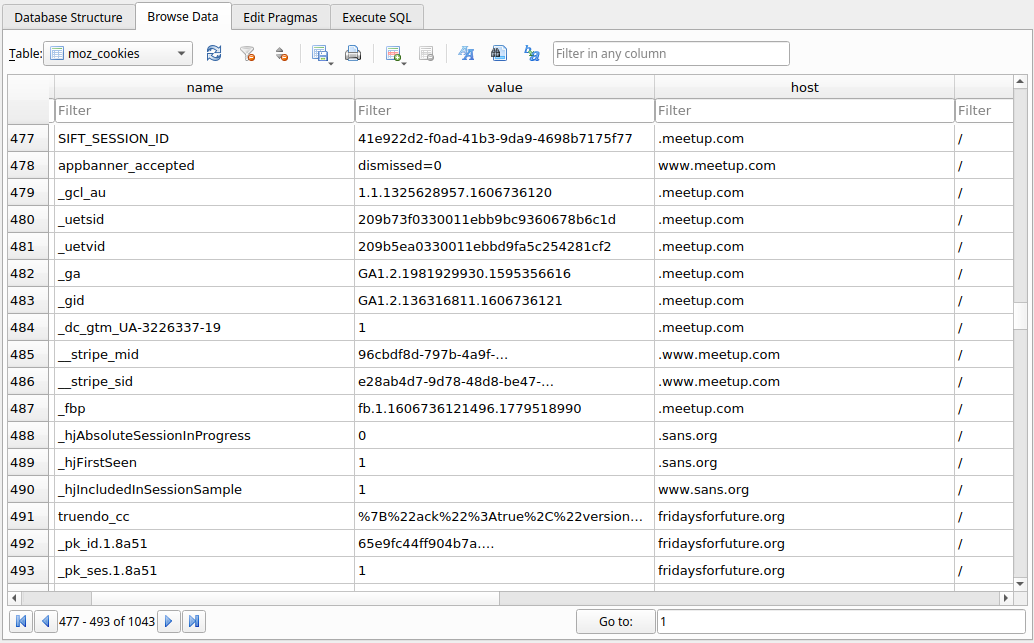
\includegraphics[width=\linewidth]{images/cookie-sqlite.png}
\label{fig:cookies}
\end{figure}

In its essence, cookies are a simple per-host key-value store in the browser; it's up to the web site to define which keys it wants to store. If a web site accesses it's own entries (as defined in the hosts column), that's called first-party data, or first-party cookies and could be used for session persistence, as seen in the first column.

If a web site accesses data from another site, that's when we're talking about third-party data, or third-party cookies which is used to track users on their visits across different web sites.

In addition to tracking in the web browser, there's also tracking in E-Mail\footnote{See \textit{Doffmann, Z. (2021)}: Why You Suddenly Need To Delete Gmail On Your iPhone \cite{deleteGmail}}, which we will not cover in this paper.

\subsection{Data Types}

\subsubsection{First-Party Data}

Now that we have covered cookies as a mechanism to persist data in the user's browser, we need to look at the various classes of data. The definition for first party data is actually quite simple, it is data that we collect from our own sources.\footnote{See \textit{OnAudience (2019)}: What is first party data? \cite{firstParty}} Data could include information that we retrieve from our own cookies or from any information the user might have left on our website, for example by looking at an item.

In e-Commerce, a common use case would be to follow up on an abandoned sale, where the user looked at an item but did not put it into their shopping cart:

\begin{figure}[H]
\centering
\caption {Don't Wait}
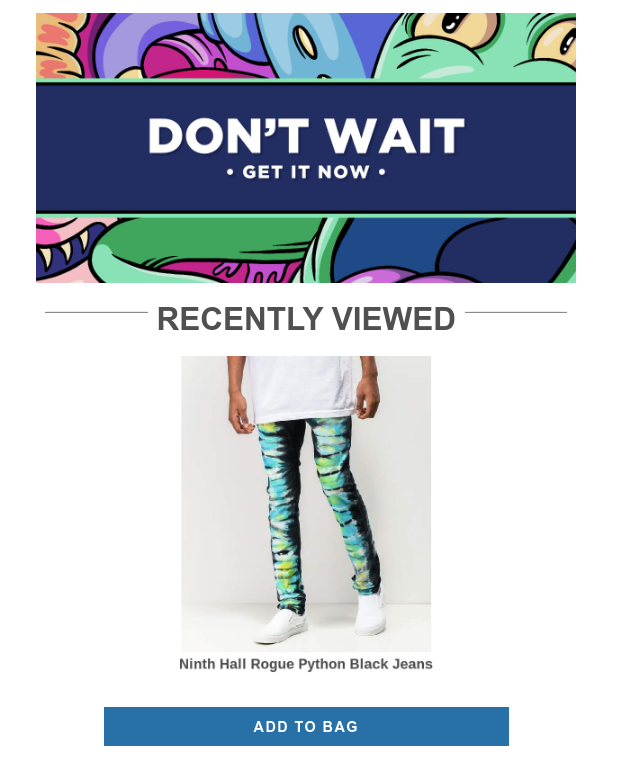
\includegraphics[width=\linewidth]{images/zumiez-dont-wait.png}
\label{fig:zumiez}
\end{figure}

This screenshot was taken from an E-Mail by \href{https://www.zumiez.com/}{Zumiez}; another example of clever use of first-party data are the regular notifications from \href{https://www.netflix.com/de-en/}{Netflix} to finish the season of a series you just started.

\subsubsection{Second-Party Data}

Second party data is another companies first party data.\footnote{See \textit{OnAudience (2019)}: What is first party data? \cite{firstParty}}

\subsubsection{Third-Party Data}

Third party data is additional data that you buy from specialized sources on the web to enrich your own data.\footnote{See \textit{OnAudience (2019)}: What is first party data? \cite{firstParty}}

- auch bei 2.2.3 würde ich mir mehr „Futter“ wünschen - was macht Third Party Cookies so besonders? Warum gibt es hier viel Diskussion zu?

—> gerade in Kapitel 2 musst du es schaffen, jemandem der sich noch nie mit dem Thema beschäftigt hat, das Gefühl eines Überblicks und einer Einführung geben. Grundlagendefinitionen und Erklärungen.

\subsection{Tool-stack - Analytics}

\subsubsection{Google Analytics}

\href{https://analytics.google.com/}{Google Analytics} gives you all the tools to analyze your web business data and gain insights into your campaign performances.

- 2.3.1 - auch hier: du gibst eine Definition, fine. Aber danach gib dem Leser noch was an die Hand. ZB wie verbreitet ist das Tool, wer nutzt es?

\subsubsection{Open Source Analytics}

In addition to Google Analytics, there are a couple of open source alternatives, one of which is Plausible.\footnote{See \textit{Frank, C. (2020)}: Usefulness of open-source tools for web analytics in EMarketing \cite{previousPaper}} 

\begin{figure}[H]
\centering
\caption {Plausible}
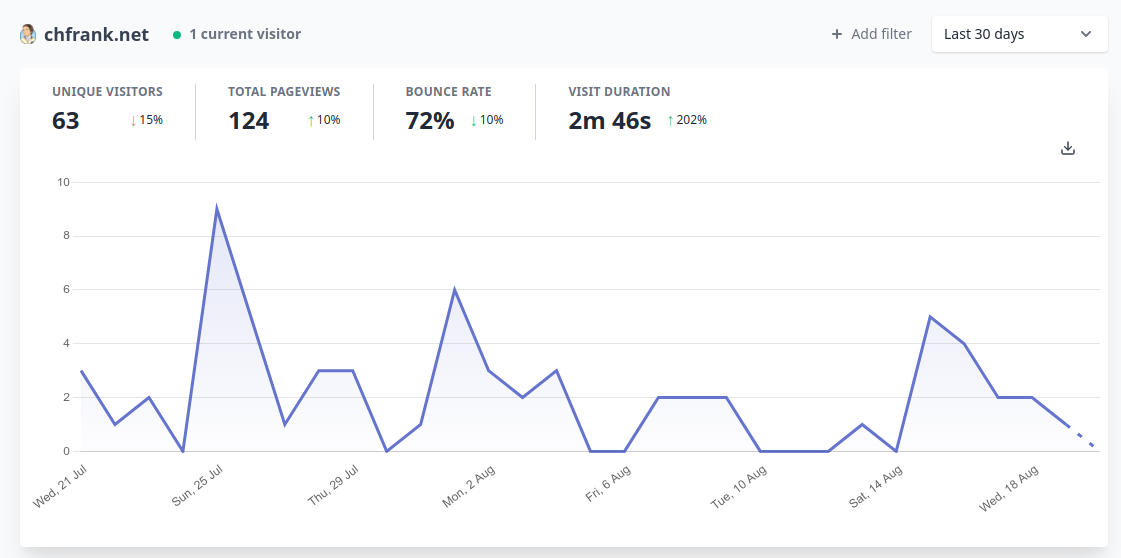
\includegraphics[width=\linewidth]{images/plausible.png}
\label{fig:plausible}
\end{figure}

Looking at the data provided, we can gather deep insights into the visitors of our page and predict the performance of our campaigns.\footnote{See \textit{Frank, C. (2021)}: Web Traffic Analysis - Predicting Blog Post Performance \cite{previousBigdata}}

We can also analyze key performance indicators for our campaigns, such as Click-Through or Conversion rates.\footnote{See \textit{Romes, Y. (2020)}: 10 Inbound KPIs, die jetzt auch Personaler kennen sollten \cite{inboundKPI}}

\subsubsection{Yandex Metrica}

\href{https://metrica.yandex.com/}{Yandex Metrica} is another commercial option for web page analytics, located in Russia.

\subsection{Tool-stack - Advertising}

\subsubsection{Google Ads}

\href{https://ads.google.com/home/}{Google Ads} is a platform to place ads on Google's pages and affiliates.

Placement and Algorithm is a science unto itself; recently Google has come under scrutint from the regulators and in one case, agreed to the ruling and the fine.\footnote{See \textit{Burgess, M. (2021)}: France Cracked Down on Google’s Ad Tech \cite{googleAds}}

- 2.4: evtl macht es hier Sinn, sich nicht in zu starke Untergliederungen zu verlieren - fasse lieber das, was du sagen möchtest in einem kurzen Abschnitt zusammen (Schwerpunktsetzung ist ein wichtiges Kriterium bei der Bewertung)

\subsubsection{Amazon Advertising}

\href{https://advertising.amazon.com//}{Amazon Advertising} is a platform to place ads for your products on Amazon's pages.

\subsubsection{Facebook Advertising}

\href{https://www.facebook.com/business/ads}{Facebook Ads} is a platform to place ads on Facebook's pages and affiliates.

\subsection{Moving past cookies}

\subsubsection{Browser-based}

To continue with targeted advertising, even after the demise of the tracking cookie, a new concept of Privacy Preserving Advertising has emerged.\footnote{See \textit{Rescorla, E. (2021)}: The future of ads and privacy \cite{futureAds}}

The primary contender in this space is \href{https://wicg.github.io/floc/}{Google FLoC}, which is under fire from a privacy point of view.\footnote{See \textit{Rescorla, E. (2021)}: Privacy analysis of FLoC \cite{privacyFloc}} Among others, EFF has published a detailed analysis of FLoC's shortcomings in regards to privacy and why they believe that FLoc would be a terrible idea.\footnote{See \textit{Cyphers, B. (2021)}: Google’s FLoC Is a Terrible Idea \cite{terribleIdea}}

\subsubsection{Data-based}

A second approach is based around data clean rooms, to enable the combination of first party data with second party data, without running afoul of data protection regulations.\footnote{See \textit{Younger, M. (2019)}: The Three Hidden Technology Trends Behind Data Clean Rooms \cite{cleanRoom}}

\subsubsection{Identity-based}

Similar to FLoC are several other approaches to implement some kind of advertising ID, that would attempt to not violate the user's privacy rights but still allow for targeted advertising. The most promising approach was Apple's ID for Advertising, which seems to be not going anywhere for the time being.\footnote{See \textit{Ray, O. (2020)}: What is IDFA and Why Apple Killed it \cite{cleanRoom}}

\subsubsection{Content-based targeting}

In 2020, the public radio in The Netherlands went from targeted advertising to contextual advertising and saw their ad revenues grow.\footnote{See \textit{Edelman, G. (2020)}: Can Killing Cookies Save Journalism? \cite{killingCookies}} 

The system at \href{https://over.npo.nl/}{NPO} is a bidding system similar to Google Ads, however, ads are not placed based on a user profile but the current context, i.e. a web page shown or a TV show watched.

\subsection{Legal Framework}

There's a number of legal frameworks that govern tracking and advertising, here's a list of the most common ones with links to the legal texts:

\begin{itemize}
 \item \href{https://gdpr-info.eu/}{GDPR} (General Data Protection Regulation)
 \item \href{https://www.datenschutz-grundverordnung.eu/}{DSGVO} (Datenschutzgrundverordnung)
 \item \href{https://dsgvo-gesetz.de/ttdsg/}{TTDSG} (Telekommunikations-Telemedien-Datenschutz-Gesetz (Entwurf ))
 \item \href{https://oag.ca.gov/privacy/ccpa}{CCPA} (California Consumer Privacy Act)
 \item \href{https://www.lgpdbrasil.com.br/}{LGPD} (Lei Geral de Proteção de Dados Pessoais)
 \item \href{https://popia.co.za/}{POPIA} (Protection of Personal Information Act)
 \item \href{https://ec.europa.eu/info/strategy/priorities-2019-2024/europe-fit-digital-age/digital-services-act-ensuring-safe-and-accountable-online-environment_en}{DSA} (Digital Services Act)
 \item \href{https://ec.europa.eu/info/strategy/priorities-2019-2024/europe-fit-digital-age/digital-markets-act-ensuring-fair-and-open-digital-markets_en}{DMA} (Digital Markets Act)
\end{itemize}

In this paper, we will assume that the reader is familiar with the content of the various regulations and solely focus on their impact and interpretation.

- 2.6: hier würde ich empfehlen, entweder die konkreten Stellen zu benennen oder die Auflistung wegzulassen und durch einen kleinen Text zu ersetzen, der deutlich macht, welche Rechtsquellen besonders wichtig und welche ergänzend wichtig sind

